\documentclass[a4paper,10pt,english]{scrartcl}
\usepackage[english]{babel}
\usepackage{iftex}
\ifXeTeX
  \usepackage{fontspec}
  \usepackage{xeCJK} % Chinese characters in Examples 8 and 10
  \setCJKmainfont{Songti SC}
  \setCJKmonofont{Songti SC}
  \newenvironment{cjktext}{}{}
\else
  \usepackage[T1]{fontenc}
  \usepackage[utf8]{inputenc}
  \usepackage{CJKutf8} % Chinese characters in Examples 8 and 10
  \newenvironment{cjktext}{\begin{CJK}{UTF8}{bsmi}}{\end{CJK}}
\fi
\usepackage[a4paper,margin=2.5cm,footskip=0.5cm]{geometry}

% Die nächsten drei Felder bitte anpassen:
\newcommand{\Aufgabe}{Task 1: Jewelry Messages} % Task number and name
\newcommand{\TeilnahmeId}{73974}                  % Teilnahme-ID angeben
\newcommand{\Name}{Hans Sihan Zhu}             % Name des Bearbeiter / der Bearbeiterin dieser Aufgabe angeben


% Kopf- und Fußzeilen
\usepackage{scrlayer-scrpage, lastpage}
\setkomafont{pageheadfoot}{\large\textrm}
\lohead{\Aufgabe}
\rohead{Participant ID: \TeilnahmeId}
\cfoot*{\thepage{}/\pageref{LastPage}}

% Position des Titels
\usepackage{titling}
\setlength{\droptitle}{-1.0cm}

% Für mathematische Befehle und Symbole
\usepackage{amsmath}
\usepackage{amssymb}
\usepackage{caption}
\usepackage{subcaption}
\usepackage{amsthm}
\newtheorem{theorem}{Theorem}
\newtheorem{lemma}[theorem]{Lemma}

% example box
\usepackage{tcolorbox}
\usepackage{xcolor}

% Für Bilder
\usepackage{graphicx}

% Für Algorithmen
\usepackage{algpseudocode}

% Für Quelltext
\usepackage{listings}
\usepackage{color}
\definecolor{mygreen}{rgb}{0,0.6,0}
\definecolor{mygray}{rgb}{0.5,0.5,0.5}
\definecolor{mymauve}{rgb}{0.58,0,0.82}
\lstset{
  keywordstyle=\color{blue},commentstyle=\color{mygreen},
  stringstyle=\color{mymauve},rulecolor=\color{black},
  basicstyle=\footnotesize\ttfamily,numberstyle=\tiny\color{mygray},
  captionpos=b, % sets the caption-position to bottom
  keepspaces=true, % keeps spaces in text
  numbers=left, numbersep=5pt, showspaces=false,showstringspaces=true,
  showtabs=false, stepnumber=2, tabsize=2, title=\lstname
}
\lstdefinelanguage{JavaScript}{ % JavaScript ist als einzige Sprache noch nicht vordefiniert
  keywords={break, case, catch, continue, debugger, default, delete, do, else, finally, for, function, if, in, instanceof, new, return, switch, this, throw, try, typeof, var, void, while, with},
  morecomment=[l]{//},
  morecomment=[s]{/*}{*/},
  morestring=[b]',
  morestring=[b]",
  sensitive=true
}
\lstset{
  language=[ISO]C++,
  % … your other styling options …
}
% Define a custom tcolorbox style for examples
\tcbset{
    % Define a counter for examples that resets within sections
    example/.style={
        colback=blue!5,
        colframe=blue!75!black,
        fonttitle=\bfseries,
        % Adjusted title to include section number
        title={Example~\thesection.\thetcbcounter},
        boxrule=0.8pt,
        arc=4pt,
        outer arc=4pt,
        boxsep=5pt,
        left=5pt,
        right=5pt,
        top=5pt,
        bottom=5pt
    },
}

% Define a new environment for examples with numbering within sections
\newtcolorbox[auto counter]{examplebox}[1][]{
    example,
    #1
}

% Diese beiden Pakete müssen zuletzt geladen werden
\usepackage[hidelinks]{hyperref} % Anklickbare Links im Dokument
\usepackage{cleveref}

% Daten für die Titelseite
\title{\textbf{\Huge\Aufgabe}}
\author{\LARGE Participant ID: \LARGE \TeilnahmeId \\\\
	    \LARGE Author: \\ 
	    \LARGE \Name\\\\}
\date{\LARGE Submitted April 2025 \\ Revised October 2026}

\begin{document}

\maketitle
\tableofcontents

\vspace{0.5cm}

\section{Problem Restatement}\label{sec:problem}

We have a necklace whose letters are coded as sequences of colored pearls, with a prefix-free code so that the message can be recovered. The problem consists of two scenarios:

a) $r$ colors all with the same diameter (length)

b) colors with different (integer) diameters

Formally, given the number of occurrences of each letter $f_i$, we wish to devise an algorithm to produce the code scheme $c_i$ so that the function

$$
\sum_i f_i \cdot \text{len}(c_i)
$$

is minimized. 

The input is the number of colors and their diameters, plus a text (`schmuck*.txt'). The output is the optimal code table plus the total encoded length it produces for the text \cite{BWINF2025}. 

\section{Solution Idea}\label{sec:idea}

In this paper, we consider the pearls of the task as encoding characters, and we use $r$ instead of $n$ to denote the number of distinct encoding characters. Our goal is to find the optimum encoding scheme of $r$ encoding characters that gives a prefix-free code for each letter (Unicode character) of the message, for both the unweighted and weighted case. Throughout, a \emph{letter} is a character of the message and an \emph{encoding character} is a pearl color; note that in the literature's term ``unequal letter costs'' \cite{GolinRote1998}, the ``letters'' are our encoding characters.

We first introduce the classic Huffman encoding algorithm for two encoding characters, and extend it to $r$ encoding characters. Then, we follow Golin and Rote's 1998 paper \cite{GolinRote1998}, explaining their ``simple algorithm'' and then the optimized one through pruning, which runs in $O(n^{C+2})$ time. In the end, we only implement the pruned, optimized algorithm, which can solve test cases from both parts a) and b).

We also acknowledge the distribution of work: the conventions of filled trees, levels and signatures, and DP were formulated by Golin and Rote; the reduction and the $O(n^{C+2})$ main algorithm were also proposed by them. They also suggest representing signatures with the strictly increasing vector, leading to the count $$\binom{n+C+1}{C+1}$$. The explicit ranking and unranking algorithms, rebuilding the actual code table from the $q_i$, full implementation details and the 10 examples were by the author.

\subsection{Huffman Encoding and its Extension}\label{sec:huffman}

We first consider the following problem, or rather, the special case of part a) when $r = 2$. Let $n$ be the number of distinct letters we want to encode (here a letter is any Unicode character of the message) and $W = \{w_1, w_2, \cdots, w_n\}$ is the set of letters, sorted in descending order by their frequencies ($w_1$ is the most frequent). We define $1> p_1 \ge p_2 \ge \cdots \ge p_n > 0$ to be the frequencies of the corresponding letters. Also, let $l_1, \cdots, l_n$ be the lengths of the codes for the letters.

We wish to minimize $Cost = \sum_{i=1}^n p_i\,l_i$.

We introduce the concept of Huffman trees. Consider \Cref{fig:htree}.

\begin{figure}
    \centering
    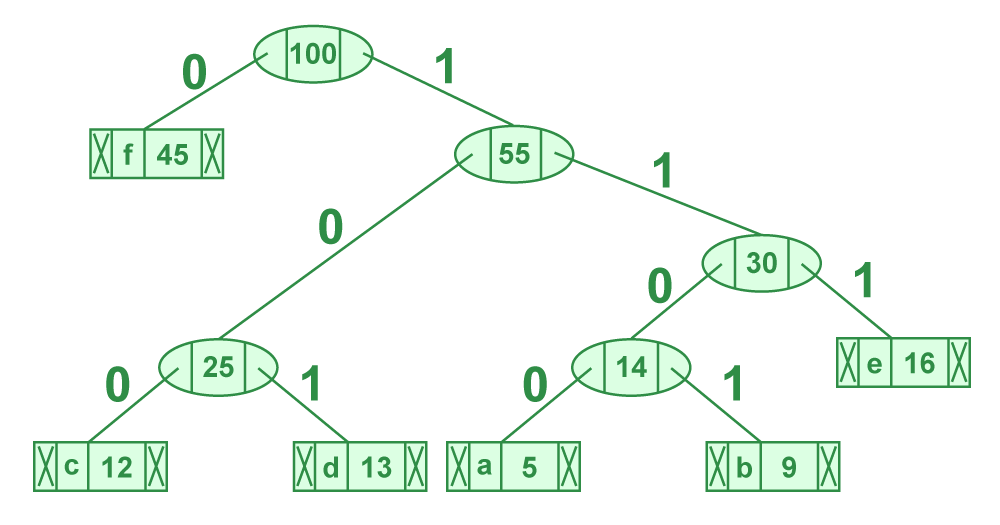
\includegraphics[width=0.75\linewidth]{Huffmantree.png}
    \caption{A valid Huffman tree encoding the characters $\{a,b,c,d,e,f\}$ with frequencies $\{0.05, 0.09, 0.12, 0.13, 0.16, 0.45\}$, in that order}
    \label{fig:htree}
\end{figure}

In a Huffman tree, each letter is embodied in a leaf in the tree, and the path of $0$'s and $1$'s taken to get to that leaf is its corresponding code. For instance, the letter $a$ is encoded with $1100$. Each node in the tree has a corresponding weight, which is the sum of all $p_i$'s of the leaves in the subtree with that node as root. Notice that no internal nodes have letters.

Huffman, in his 1952 paper \cite{Huffman1952}, proposed the following algorithm:

\begin{verbatim}
Let W be the vector of letters and p their frequencies (descending as specified)
While len(W) > 1:
    Select the last two elements of W and delete them
    Remove the two letters' frequencies from p and replace with their sum*
    Add a new letter representing the two deleted letters into W*
    Let the new letter be the direct parent of the two deleted elements
The remaining element in W is the root of the encoding tree.
\end{verbatim}

The resulting tree represents the desired encoding scheme. Notice that at *, we insert the values so that the descending property is maintained. At each point, the ``new letter'' is a non-existent representative of its two children; in other words, it is an internal node. 

We further illustrate this algorithm using the example shown in \Cref{fig:htree} above (see \Cref{tab:huffmansim}).

\begin{table}[h]
\centering
\begin{tabular}{r|c|c|l}
\hline
\textbf{Step} & \textbf{Merged Pair} & \textbf{New Weight} & \textbf{New W} \\ 
\hline
0 & — & — & 
\(\{f_{45},\,e_{16},\,d_{13},\,c_{12},\,b_{9},\,a_{5}\}\) \\[6pt]
1 & \(a_{5}+b_{9}\to (ab)_{14}\) & 14 & 
\(\{f_{45},\,e_{16},\,(ab)_{14},\,d_{13},\,c_{12}\}\) \\[6pt]
2 & \(c_{12}+d_{13}\to (cd)_{25}\) & 25 & 
\(\{f_{45},\,(cd)_{25},\,e_{16},\,(ab)_{14}\}\) \\[6pt]
3 & \((ab)_{14}+e_{16}\to (abe)_{30}\) & 30 & 
\(\{f_{45},\,(abe)_{30},\,(cd)_{25}\}\) \\[6pt]
4 & \((cd)_{25}+(abe)_{30}\to (cdeab)_{55}\) & 55 & 
\(\{(cdeab)_{55},\,f_{45}\}\) \\[6pt]
5 & \(f_{45}+(cdeab)_{55}\to (all)_{100}\) & 100 & 
\(\{(all)_{100}\}\) \\
\hline
\end{tabular}
\caption{Simulation of Huffman's greedy merging process for \Cref{fig:htree}, where the resulting tree is shown}
\label{tab:huffmansim}
\end{table}

This algorithm runs in $O(n\log(n))$.

\begin{lemma}\label{lem:monotone}
If $$p_1\ge p_2\ge\cdots \ge p_n$$ and $l_i$ is the depth of the $i$th character, the optimal code always satisfies $$l_1 \le l_2\le \cdots \le l_n.$$
\end{lemma}

\begin{proof}
Suppose that the optimal code does not satisfy $l_1 \le l_2\le \cdots \le l_n$. Then, considering a reordering of the same lengths in ascending order ($l_1' \le l_2'\le \cdots \le l_n'$) would yield a smaller $Cost$:
$$\sum_{i=1}^n p_i\,l_i \ge \sum_{i=1}^n p_i\,l_i',$$
as given by the classic Rearrangement Inequality.
\end{proof}

Ultimately, this is a greedy algorithm in which \Cref{lem:monotone} is utilized. The letters with smaller weight should always go at deeper levels, while letters with greater weights are saved to be put towards the top of the tree. The greedy is justified as follows: some optimal tree has the two least frequent letters as siblings at maximum depth, as swapping them into the deepest positions never raises the cost by \Cref{lem:monotone}; we can merge those two siblings into one letter of weight $p_{n-1}+p_n$, where the reduced problem always costs $p_{n-1}+p_n$ less than the corresponding original tree; induction on $n$ would complete the proof \cite{Huffman1952}.

Now we consider the expansion towards $r$-encoding characters. The essential idea is to repeat the same procedure as in the $r=2$ case, by repeatedly merging the least frequent $r$ elements, with correctness similarly justified after padding.

Notice that in a Huffman tree, there are always $r + (r-1)k$ leaves, where $k$ is the number of internal nodes except the root node. This is because each of the $k+1$ internal nodes (including the root node) contribute $r$ nodes, and there are $k$ nodes that are internal nodes and not leaves. Hence, there are $$leaves = total - internal = (k+1)r - k = r + (r-1)k$$ leaves in the tree.

This number, however, is not always equal to $n$, and will result in some of the very top leaves not being utilized, definitely damaging the correctness of the algorithm. To solve this problem, we pad our letters with dummy letters of $0$ frequency. Since we want $n+d = r+(r-1)k$ for some $k$ where $d$ is the number of $0$-leaves we pad, we wish for $$n + d \equiv 1 \pmod{r-1},$$ which simplifies to $$d \equiv 1-n \pmod{r-1}.$$

In this way, our algorithm would first distribute the $0$'s across the deepest layers, not affecting the total cost $$Cost \;=\;\sum_{i=1}^n p_i\,\ell_i.$$

Once all dummy letters have been ``absorbed'' into zero-weight subtrees, every remaining merge involves exactly \(r\) genuine letters and increases the cost by the sum of their frequencies, which by construction is the smallest possible among all choices of \(r\) leaves. Hence, the padded \(r\)-ary Huffman procedure indeed produces an optimal prefix-free code, as some optimal tree has the $r$ smallest weights as siblings at the deepest level. The pseudocode for the algorithm is given below:

\begin{verbatim}
Pad W, p with dummy letters of frequency 0 according to the number computed.
Let W be the vector of letters and p their frequencies (descending as specified)
While len(W) > 1:
    Select the last r elements of W and delete them
    Remove the r letters' frequencies from p and replace with their sum
    Add a new letter representing the r deleted letters into W
    Let the new letter be the direct parent of the r deleted elements
The remaining element in W is the root of the encoding tree.
\end{verbatim}

Like the $r = 2$ case, this algorithm runs in $O(n\log(n))$.

\subsection{Unequal Integer Letter Costs: the Simpler Algorithm}\label{sec:simple}

Although Bradford et al.\ \cite{Bradford2002} proposed an $O(n^{C+1})$ time algorithm for binary encoding ($r = 2$), the current best exact algorithm for general $r$ was given by Golin and Rote in 1998 in their paper ``A Dynamic Programming Algorithm for Constructing Optimal Prefix-Free Codes with Unequal Letter Costs'' \cite{GolinRote1998}. This paper will be our main source of reference for this problem. 

The main idea of the simpler algorithm is to construct filled trees from top to bottom, using dynamic programming on a tree's ``signature'' to search for the optimal value. 

Before anything else, we perform the 0-padding as mentioned before. In addition, we note that we continue to use Huffman trees, and in fact, much of the solution idea is dependent on Huffman trees. Here, the ``depth'' of each edge may differ; for instance, an encoding character of length $2$ may directly go down by two depths.

Some other commonly known terms are defined here:
\begin{itemize}
    \item Leaves are nodes that have no children.
    \item Internal nodes are nodes that are not leaves.
\end{itemize}

We start by defining a $fill(T)$ function for Huffman trees T. This $fill$ function returns a tree with the same set of internal nodes as $T$ where all internal nodes have $r$ children. 

Considering the space of all trees $T$ with $n$ leaves, we see that every $T$ has a corresponding $F= fill(T)$, and if this full tree has $m$ leaves, we have the restriction that $$n \le m \le n(r-1).$$ 

Then, conversely, all $F$ satisfying $n \le m \le n(r-1)$ must have some valid $T$ with $n$ leaves. We show this by offering a construction.

Let $I$ be the number of internal nodes of $F$. We have that $m = 1 + (r-1)I$. Solving for $I$, we have $$I = \frac{m-1}{r-1} \le \frac{n(r-1)-1}{r-1}<n,$$ giving $I \le n-1$. Then, let the internal nodes be $\{v_1,v_2, \cdots, v_I\}$. For all $v_i$ with leaf-children, we choose exactly one of the leaves to be in $T$, so that a total of at most $n-1$ leaves are chosen. We can always take extra when needed, and there will always be enough leaves to take as $m \ge n$. Hence, we have successfully constructed a $T$ for all $F$. 

This means to solve the problem, we just have to find the minimum value of the ``cost'' across $fill(T)$ with $n \le m \le n(r-1)$.

Next, we introduce the idea of levels. A tree $T$'s level is the largest $i$ such that all its internal nodes have depth at most $i$ (the root node has depth 0). Now, let $T$ be an $i$-level tree. We define its \textit{signature} as the $(C+1)$-tuple $$sig_i(T) = (m;l_1,l_2,\cdots,l_C),$$ where $C$ is the largest integer cost across the encoding characters, $m$ is the number of leaves with depth at most $i$ and $l_k$ the number of leaves at depth $i+k$.

Since all $fill(T)$ have at most $n(r-1)$ leaves, we have the constraint $$m+l_1+\cdots +l_C \le n(r-1).$$

Now, if $\{v_1, v_2, \cdots , v_n\}$ are the top leaves of a general $i$-level tree $T$, with $v_1$ being the topmost leaf (and recalling that $p_i$ are sorted in descending order), we can define the cost of a general $i$-level tree $T$ to be 

\begin{equation}\label{eq:cost}
    cost_i(T) = \begin{cases}
        \sum_{t=1}^m depth(v_t)\cdot p_t+i \sum_{t=m+1}^n p_t & m \le n,\\
        \sum_{t=1}^n depth(v_t)\cdot p_t & m \ge n.\\
    \end{cases}
\end{equation}

Notice that when $m < n$, the cost function assigns a temporary depth of $i$ to the $n-m$ letters that are not yet placed on a leaf of depth at most $i$, and when $m \ge n$, it returns the actual, correct cost of the tree $T$. This cost definition will come in handy later when transitioning. In general, the ``cost'' of a tree refers to its $cost_i$ for $i$ the tree's level.

Furthermore, we define $$Trunc_i(T) = root(T) \cup \{u \in T: depth(parent(u))\le i\},$$ which in other words, is the subtree that has all its internal nodes at or above depth $i$. 

Every $F = fill(T)$ can be constructed from top to bottom, that is, if we let $F_i = Trunc_i(F)$, we can compute information about $F_i$ from $i = 1$ to F's level. 

We consider what happens when we transition from $F_i$ to $F_{i+1}$, paying special attention to the signatures of their corresponding levels and their costs. For nodes with depth less than or equal to i, nothing changes; for nodes with depth $i+1$, in $F_{i}$, they were all leaves, but in $F_{i+1}$, some of these nodes may become internal nodes with their own children. Since $F_{i+1}$ is filled, each of these nodes will obtain exactly $r$ children.

Then, if we let $q$ of these depth $i+1$ leaves become internal nodes, we have that 
\begin{equation}\label{eq:sigtrans}
sig_{i+1}(F_{i+1}) = (m+l_1; l_2, l_3, \cdots, l_C, 0) + q(-1; d_1, d_2, \cdots , d_C),
\end{equation}
where for $(d_1, d_2, \cdots, d_C)$, we write $d_i$ as the number of encoding characters with weight $i$. The left vector represents the shift in interpretation of the original nodes when moving to $sig_{i+1}$ and the right vector represents the changing of states of depth-$(i+1)$ nodes and the addition of new leaves, which sprout from depth $i+1$ and have amount indicated by $d_i$.

This definition does not specify \textit{which} of the depth $i+1$ nodes are transformed, but only cares about amount. The exact specification of nodes is not necessary, as only depths and  the overall structure matters to us. 

Next, we consider the change in cost when moving from $cost_i(F_i)$ to $cost_{i+1}(F_{i+1})$. When $m \ge n$, the cost does not change, as stagnant in the $m \ge n$ case of the definition. Otherwise when $m \le n$, citing the original calculations given by Golin and Rote \cite{GolinRote1998} and taking $m' = m+l_1-q$ as the new $m$ for $F_{i+1}$, we have

\begin{align}
    cost_{i+1}(F_{i+1}) &= \left(\sum_{1\le t\le m} depth(v_t)p_t + \sum_{m < t \le m'} (i+1)p_t\right) + (i+1)\sum_{m'<t \le n}p_t,\\
    &= \left(\sum_{1\le t\le m} depth(v_t)p_t + i\sum_{m < t \le n} p_t\right) + \sum_{m < t \le n} p_t,\\
    &= cost_i(F_i) + \sum_{m < t \le n} p_t. \label{eq:costtrans}
\end{align}

We have successfully established a transition from $F_i$ to $F_{i+1}$ in terms of the signature and the cost. We now utilize some dynamic programming with $DP[m;l_1, l_2,\cdots ,l_C]$ being the optimal cost across all filled-trees with signature $(m;l_1, l_2,\cdots ,l_C)$.

Quite easily, with the above analysis, we could move from $DP[m;l_1, l_2,\cdots ,l_C]$ to $DP[m';l_1', l_2',\cdots ,l_C']$ by simply adding that $\sum_{m < t \le n} p_t$ term.

We now propose an order in which to visit the signatures so that every $F_i$ definitely comes before $F_{i+1}$. This order is in lexicographically increasing order of $(m+l_1+l_2+\cdots+l_C, m+l_1+l_2+\cdots+l_{C-1}, \cdots , m+l_1+l_2, m+l_1, m)$. 

Recall the signatures of $F_i$ and $F_{i+1}$. We compute the difference between their first term in this newly defined sequence:

$$\text{difference} = (m'+l_1'+l_2'+\cdots+l_C') - (m+l_1+l_2+\cdots+l_C) = q(-1+d_1+\cdots + d_C) > 0,$$

meaning that $F_i$ must always come before $F_{i+1}$ because its first index in the new sequence is always smaller. Notably, when $q = 0$, the first index is equal, but the new signature is the old one shifted left with its last entry duplicated, so it still comes later \cite[Lemma~8]{GolinRote1998}.

We now outline the simple algorithm in the following high-level pseudo-code.

\begin{verbatim}
DP[0; d1, d2, ..., dC] = 0
Loop through valid signatures in lexicographically increasing order of the previously 
proposed sequence:
    Compute the new cost when transitioning from the current (cost transition)
    For q from 0 to l1:
        Compute the new signature (signature transition)
        If this new signature is valid, update its corresponding DP value
The minimum across all DP's with m >= n is the optimal cost 
\end{verbatim}

Here the cost transition is \eqref{eq:costtrans} and the signature transition is \eqref{eq:sigtrans}. In the pseudo-code, ``valid signatures'' refers to signatures satisfying $m + l_1 + l_2+\cdots +l_C \le n(r-1)$, as mentioned. The initial value is for the tree with the root as the only internal node, with its cost computed by our defined cost function. For the final answer, we require $m \ge n$ for the filled tree to have ``matured'' into the condition that we have previously proven to have an original tree. 

Since there are $C+1$ numbers in the range of $0$ to $n(r-1)$, one upper bound of the number of DP states is $(n(r-1))^{C+1}$. Each state computes $l_1+1$ transitions, where $l_1$ can be up to $n(r-1)$. Hence, the overall complexity is $O((n(r-1))^{C+2})$.

\subsection{The Main Algorithm}\label{sec:main}

Continuing to study Golin and Rote \cite{GolinRote1998}, they propose an even faster algorithm capable of running in $O(n^{C+2})$. We will first describe their algorithm and then address the part of recovering the set of codes from the DP, as ultimately desired by the problem. 

We continue to run a DP over filled trees, but this time, we limit the sum of the signature to be at most $n$. We see that whenever $m > n$ the portion of leaves that are not top $n$ will not contribute to the cost. In other words, we only care about the top $n$ nodes, and we can compress signatures with $(m; l_1, l_2, \cdots, l_C)$ with $m+l_1+\cdots+l_C>n$ to a signature with sum within $n$, to run a DP within a smaller space. 

We formalize the process of throwing away the deep leaves and only keeping the $n$ top leaves as $Reduce(T)$, which is the smallest subtree containing the root and the top $n$ leaves. 

Now, when transitioning from $F_i$ to $F_{i+1}$, the change in cost is the same as before, but the change in signature needs modification. 

We represent the new signature with $reduce(S) = sig_i(Reduce(T))$, where $S = sig_i(T) = (m; l_1, l_2, \cdots, l_C)$ with $m+l_1+\cdots+l_C>n$. We have that $m' = \min(m,n)$, and for each $j = 1, \cdots, C$, we have 
\begin{equation}\label{eq:reduce}
l'_j = \min\left(l_j,\ n-\left(m'+\sum_{k=1}^{j-1} l'_k\right)\right).
\end{equation}

This second possibility in the minimum function denotes essentially the number of nodes ``left'' from the $n$ maximum after its previous layers. Under this computation, all original signatures with sum greater than $n$ would become signatures with sum equal to $n$. Since cost is computed with the top $n$, this does not affect the cost of the signature itself, neither the following signatures that it produces, as only children of the top $n$ leaves could have the possibility of contributing.

Golin and Rote \cite{GolinRote1998} note that now, however, it is possible to have reverse edges in the lexicographically increasing order, but they reason that an optimal tree never takes a reverse edge. 

Let $T$ be an optimal tree, and $T_i = Trunc_i(T)$ and $T_i' = Reduce(Fill(T_i))$. Let $Expand_i(F,q)$ denote the tree obtained from $F$ by turning $q$ of its leaves at depth $i+1$ into internal nodes, each with all $r$ children. We have
\begin{align*}
    T'_{i+1} &= Reduce(Fill(T_{i+1})),\\
    &= Reduce(Expand_i(Fill(T_i), q_i)),\\
    &= Reduce(Expand_i(T_i', q_i)),
\end{align*}

where the second equality holds because both sides are full trees with the same internal nodes on every level and the third holds because reducing before and after the expansion gives the same tree, as shown by Golin and Rote \cite[Lemma~10]{GolinRote1998}.

Letting $k$ be the height (or depth) of $T_i'$, we consider $$S_i = sig_i(T_i') = (m; l_1, l_2, \cdots, l_C)$$ and $$S_{i+1} = sig_{i+1}(T_{i+1}') = (m'; l_1', l_2', \cdots, l_C').$$ We see that $m+l_1+\cdots + l_C = m+l_1+\cdots + l_{C-1} = \cdots = m+l_1+\cdots + l_{k-i} = n$ and $m+l_1+\cdots + l_{k-i-1} < n$. Golin and Rote use this, together with the fact that every internal node of an optimal tree has at least two children \cite[Lemma~2]{GolinRote1998}, to show that $S_{i+1}$ always comes after $S_i$ in the lexicographic order \cite[Lemma~10]{GolinRote1998}; that is, the optimal tree never takes a reverse edge. 

Hence, the lexicographically increasing order of signatures still produces the optimal value, and we outline our main algorithm's pseudocode (a more precise version as given by Golin and Rote \cite{GolinRote1998}):

\begin{verbatim}
DP[reduce(0; d1, d2, ..., dC)] = 0, set others to infinity
Loop through valid signatures in lexicographically increasing order of 
(m+l1+l2+...+lC, m+l1+l2+...+l(C-1), ..., m+l1+l2, m+l1, m):
    Compute the new_cost when transitioning from the current (cost transition)
    For q from 0 to l1:
        Compute S = the new signature (signature transition)
        If the sum of this S > n, replace with reduce(S)
        Set DP[S] = min(DP[S], new_cost)
DP[n; 0, ..., 0] is the optimal cost 
\end{verbatim}

Here the cost transition is \eqref{eq:costtrans}, the signature transition is \eqref{eq:sigtrans}, and the reduction is \eqref{eq:reduce}. $DP[n; 0, \ldots, 0]$ itself is the optimal answer, as maintained to be the place where all ``fully-grown'' filled trees meet.

The time complexity of this algorithm is $O(n^{C+2})$ by a similar analysis as before. Specifically, we compute the number of states we need to visit, which is the number of tuples with $C+1$ nonnegative integers with sum at most $n$. A classic trick in olympiad math as well, we have that $$(m, m+l_1+1, m+l_1+l_2+2, \cdots , m+l_1+\cdots+l_C+C)$$ is strictly increasing. And this new sequence forms a one-to-one correspondence to the original sequence. The largest possible value of $m+l_1+\cdots+l_C+C$ is $n+C$, while the smallest value of $m$ is 0. So, the number of possible signatures is just $$\binom{n+C+1}{C+1},$$

on which our space complexity is dependent on.

When implemented, we would realize that many of these $\binom{n+C+1}{C+1}$ signatures are ultimately not visited, and so, we can simply choose to skip over them.

Finally, for each signature, we can record the previous signature that resulted in the best solution, as well as the $q$ taken to reach that signature. Then, we can easily backtrack and find the $q_i$ taken at each stage. Let $j$ be the level of the optimal tree.

To recover the original tree, we start with the tree with the root node as the only internal node and at each level $i$, starting from 1 and ending at $j$, expand $q_i$ leaves at that level as from the backtracking. We elaborate more on this in the implementation section.

Finally, despite much literature on this problem \cite{Karp1961, GolinKenyonYoung2002, GolinLi2008}, with Golin and Rote \cite{GolinRote1998} being by far the best exact solution and various other approximation algorithms, we have not determined yet whether this problem is NP-hard, nor have we devised any polynomial-time exact algorithm.

\section{Implementation}\label{sec:impl}

When implementing the algorithm, the biggest difficulty to resolve is that of compressing the signatures to a one-dimensional array that is easy to access, as well as devising a method that can do so in reverse. In my program, these functions are called indexOf() and signatureOf(idx), respectively (the input and output are done on global arrays).

Specifically, indexOf() for an input array of the signature returns the 1-based index at which the signature appears in the lexicographically increasing order. To do this, we recall that $$(m+l_1+\cdots+l_C+C,\ m+l_1+\cdots+l_{C-1}+(C-1),\ \ldots,\ m+l_1+1,\ m)$$ is strictly decreasing, and its lexicographically increasing order maps perfectly to the lexicographically increasing order of $(m+l_1+\cdots+l_C,\ m+l_1+\cdots+l_{C-1},\ \ldots,\ m+l_1,\ m)$ by a difference of $(C, C-1, \cdots, 2, 1, 0)$. 

Then, for a given signature we simply find the index at which $S = (m+l_1+\cdots+l_C+C,\ m+l_1+\cdots+l_{C-1}+(C-1),\ \ldots,\ m+l_1+1,\ m)$ appears. Another way to view this sequence is choosing $C+1$ elements out of $n+C+1$, as previously noted. We can denote the presence of each number by using a binary number of $n+C+1$ digits, where $1$ means the index of its digit is chosen in S. 

To find this index, we consider at each $1$ the number of binary numbers that came before it. If we have a $1$ on the $i$th digit (from the right, 0-indexed) and previously placed $k$ 1's (to the left), this $1$ on the $i$th digit puts it after all the binary numbers with the same portion before the $i$th digit and with a $0$ on the $i$th digit. Those number of those binary numbers can be written as $$\binom{i}{C+1-k}.$$ Hence, this allows us to scan our binary number from left to right, and add this corresponding amount at each $1$. Finally, we add one to obtain the index of our number itself. In pseudo-code,

\begin{verbatim}
Set idx = 0, S as defined earlier.
For j from 0 to C:
    Increase idx by (S[j] choose C+1-j)
return idx + 1
\end{verbatim}

Here, j directly loops over the 1's, and $S[j]$ is the corresponding element in $(m+l_1+\cdots+l_C+C,\ m+l_1+\cdots+l_{C-1}+(C-1),\ \ldots,\ m+l_1+1,\ m)$, which perfectly happens to be the number of digits to the right, and in descending order. We also precompute the combination numbers.

When going in reverse and given the index, at each place from $n+C$ to 0, we consider how many binary numbers our number would follow if we place a $1$ there. If that number is greater or equal to our index, we cannot afford to put a 1, otherwise, we select that digit to be 1. This method is embodied in the following pseudocode:

\begin{verbatim}
Set idx = given index - 1, S is empty and will be recovered.
For i from n+C to 0:
    If idx >= comb[i][C+1-used]:
        idx -= comb[i][C+1-used]
        S[used] = i
        If used > C Done
\end{verbatim}

The used variable records the number of $1$'s previously expended. This algorithm first recovers the $S$ array, from which the original array can be easily devised.

To recover the original tree, we maintain an array of sets of strings representing the code strings with a certain cost. Specifically, $buckets[cost]$ is a set of strings with cost $cost$. Recalling that for each $i$ from 1 to $j$, we expand $q_i$ of the $i$-level leaves, we select $q$ strings from buckets[i] and for each string $s$, for each encoding character $c$, we add $s+c$ to the corresponding bucket. When complete, we delete those $q$ strings.

Then finally, for output, we select the $n$ cheapest code strings and assign them to the letters in order of decreasing frequency by climbing up $buckets[cost]$ and taking all at each layer until we can't.

We previously mentioned that to speed up the process, it is possible to skip over some states directly. This motivates us to consider a BFS-style approach that uses a data-structure to maintain the next smallest signature that we plan on visiting. In this way, we could avoid storing data for every signature and save time iterating. However, an actual implementation of this approach on the last test case, which is the only one that doesn't succeed, shows that this is similarly unsuccessful. Therefore, we choose to keep our original main algorithm for simplicity (the extra maintenance of the multiset data structure ends up damaging time for easier cases).

\section{Examples}\label{sec:examples}

Unfortunately, even with a queue optimization that allows direct skipping over some states, our code is unable to process \texttt{schmuck9.txt} within a reasonable amount of time. The combination number has spiked to around $1.2\times 10^{12}$, rendering it almost impossible. \Cref{tab:runtime} shows the results of running the implementation.

\begin{table}[h]
\centering
\caption{State space and running time of the implementation (Apple M4, \texttt{g++ -O2}, median of 5 runs; $n$ includes the zero-weight padding letters).}
\begin{tabular}{lrrrrrr}
\hline
Example & $r$ & $C$ & $n$ & $\binom{n+C+1}{C+1}$ & visited & time \\
\hline
\texttt{schmuck0}  & 2  & 1 & 12  & 91            & 50        & $<$1 ms \\
\texttt{schmuck00} & 3  & 1 & 29  & 465           & 101       & $<$1 ms \\
\texttt{schmuck01} & 5  & 1 & 45  & 1{,}081       & 95        & $<$1 ms \\
\texttt{schmuck1}  & 3  & 2 & 25  & 3{,}276       & 262       & $<$1 ms \\
\texttt{schmuck2}  & 2  & 5 & 9   & 5{,}005       & 350       & $<$1 ms \\
\texttt{schmuck3}  & 3  & 3 & 9   & 715           & 50        & $<$1 ms \\
\texttt{schmuck4}  & 2  & 5 & 14  & 38{,}760      & 1{,}834   & $<$1 ms \\
\texttt{schmuck5}  & 7  & 6 & 43  & 99{,}884{,}400 & 2{,}905  & 38 ms \\
\texttt{schmuck6}  & 3  & 3 & 35  & 82{,}251      & 1{,}993   & $<$1 ms \\
\texttt{schmuck7}  & 10 & 4 & 82  & 36{,}949{,}857 & 1{,}568  & 27 ms \\
\texttt{schmuck8}  & 5  & 3 & 321 & 456{,}326{,}325 & 1{,}059{,}999 & 909 ms \\
\texttt{schmuck9}  & 4  & 4 & 676 & $\approx 1.20\times10^{12}$ & --- & not feasible \\
\hline
\end{tabular}
\label{tab:runtime}
\end{table}

Importantly, time is dominated by scanning the whole table of $\binom{n+C+1}{C+1}$ entries, even though only a small fraction of it is ever visited. 

\subsection{Example 1}\label{ex:1}

\textbf{Input:} \texttt{schmuck0.txt}

\textbf{Output:}

\begin{verbatim}
113
E 122
  211
N 212
I 221
S 222
R 1112
O 1121
M 1122
L 1211
D 1212
H 11111
C 11112
Elapsed time: 0 ms
\end{verbatim}

\textbf{Commentary:} This successfully achieves the minimum as given in the problem document. The code given is one of the many possible optimal codes. 

\subsection{Example 2}\label{ex:2}

\textbf{Input:} \texttt{schmuck1.txt}

\textbf{Output:}

\begin{verbatim}
191
e 3
t 13
  211
w 212
r 221
n 222
i 23
s 1121
f 1122
b 113
I 1211
B 1212
" 1221
ü 1222
u 123
o 213
m 223
k 11111
h 11112
d 11121
a 11122
W 1113
N 1123
F 1213
D 1223
Elapsed time: 0 ms
\end{verbatim}

\textbf{Commentary:} We see that the algorithm correctly orders the most frequent to take the least weighted code.

\subsection{Example 3}\label{ex:3}

\textbf{Input:} \texttt{schmuck01.txt}

\textbf{Output:}

\begin{verbatim}
1150
  4
e 5
n 15
r 21
i 22
...
Elapsed time: 0 ms
\end{verbatim}

\textbf{Commentary:} Implementing the Huffman encoding algorithm for $r>2$ characters would yield the same optimal cost. We see that the algorithm correctly orders the most frequent, the space character, to take the least weighted code. 

\subsection{Example 4}\label{ex:4}

\textbf{Input:} \texttt{schmuck2.txt}

\textbf{Output:}

\begin{verbatim}
135
a 1
h 2111111
g 212
f 221
e 2112
d 21112
c 211112
b 2111112
  222
Elapsed time: 0 ms
\end{verbatim}

\textbf{Commentary:} Manually drawing a Huffman tree and summing up the depths times frequencies, we have $33+11+12+13+14+15+11+11+15 = 135$, so, at least the calculation is right. In addition, we observe that the program assigned the code ``1'' to the letter ``a'', with frequency 33, which makes sense because its frequency is significantly greater than others. For instance, when placed under a $5$, the a's would immediately yield $5 \cdot 33 = 165$, exceeding this cost.

\subsection{Example 5}\label{ex:5}

\textbf{Input:} \texttt{schmuck3.txt}

\textbf{Output:}

\begin{verbatim}
279
c 11
b 2
a 3
  13
h 1211
g 122
f 1212
e 123
d 1213
Elapsed time: 0 ms
\end{verbatim}

\textbf{Commentary:} An analysis similar to \hyperref[ex:4]{Example 4} can be performed, leaving us with relative confidence that the code is doing its job correctly. Compared to the previous example, we see this solution is more ``balanced'' in its tree, where no character is favored significantly more over others, as against the ``a'' character previously.

\subsection{Example 6}\label{ex:6}
\textbf{Input:} \texttt{schmuck4.txt}

\textbf{Output:}

\begin{verbatim}
137
n 211
m 11111111
l 1112
k 1121
j 1211
i 11112
h 111112
g 22
f 1111112
e 122
d 212
c 11111112
b 1122
a 1212
Elapsed time: 1 ms
\end{verbatim}

\textbf{Commentary:} Considering the ``balancedness'' again, we see that in this test case, the frequencies of all the letters are equal, and hence, this tree is quite balanced indeed: the smallest weight being 7 and the largest 12. 

\subsection{Example 7}\label{ex:7}
\textbf{Input:} \texttt{schmuck5.txt}

\textbf{Output:}
\begin{verbatim}
3162
  22
e 3
t 111
i 112
o 121
s 122
a 13
n 211
...
Elapsed time: 54 ms
\end{verbatim}

\textbf{Commentary:} This test case has the largest maximum cost among the examples ($r = 7$, $C = 6$), so its table of $\binom{50}{7} \approx 10^8$ signatures is by far the largest relative to $n$ (\Cref{tab:runtime}); nevertheless only 2{,}905 signatures are visited.

\subsection{Example 8}\label{ex:8}
\textbf{Input:} \texttt{schmuck6.txt}

\textbf{Output:}

\begin{cjktext}
\begin{verbatim}
234
， 31
馬 113
有 1211
文 122
...
Elapsed time: 1 ms
\end{verbatim}
\end{cjktext}

\textbf{Commentary:} This is an example where the algorithm could be extended to a larger set of unicode that are less commonly seen in English or German-speaking countries. 

\subsection{Example 9}\label{ex:9}
\textbf{Input:} \texttt{schmuck7.txt}
\textbf{Output:}

\begin{verbatim}
134559
  4
e 5
n 6
i 7
...
Elapsed time: 30 ms
\end{verbatim}

\subsection{Example 10}\label{ex:10}
\textbf{Input:} \texttt{schmuck8.txt}
\textbf{Output:}

\begin{cjktext}
\begin{verbatim}
3287
， 42
。 5
」 242
...
Elapsed time: 1013 ms
\end{verbatim}
\end{cjktext}


\section{Source Code}\label{sec:code}

The indexOf() function as mentioned in the implementation section:

\begin{lstlisting}
long long indexOf() {
    int t[C+1];
    t[C] = inSign[0];
    for (int i = C-1; i >= 0; i--){
        t[i] = t[i+1]+inSign[C-i]+1;
    }
    // t = m+l1+...+lC+C,m+l1+...+l(C-1)+C-1,... m+l1+1, m
    long long idx = 0;
    for (int i = 0; i <= C; i++){
        idx += comb[t[i]][C+1-i];
    }
    return idx + 1;
}
\end{lstlisting}

The signatureOf() function as mentioned in the implementation section:

\begin{lstlisting}
void signatureOf(long long ind) {
    long long idx = ind-1;
    // first recover t
    // t = m+l1+...+lC+C,m+l1+...+l(C-1)+C-1,... m+l1+1, m
    int t[C+1];
    int used = 0;
    for (int i = n+C; i >= 0; i--){
        if (idx >= comb[i][C+1-used]){
            idx -= comb[i][C+1-used];
            t[used] = i;
            used++;
            if (used > C) break;
        }
    }
    outSign[0] = t[C];
    for (int i = 1; i <= C; i++){
        outSign[i] = t[C-i]-t[C-i+1]-1;
    }
    return;
}
\end{lstlisting}

The reduce() function reducing the signature:

\begin{lstlisting}
void reduce(int m){
    int mp = min(m, n);
    inSign[0] = mp;
    int ts = 0;
    for (int i = 1; i <= C; i++){
        inSign[i] = min(inSign[i],n-mp-ts);
        ts += inSign[i];
    }
}
\end{lstlisting}

The main DP loop that yields the answer:

\begin{lstlisting}
outSign[C+1] = 0;
// initialize first dp value:
inSign[0] = 0;
for (int i = 1; i <= C; i++){
    inSign[i] = d[i];
}
reduce(0);
int initialIdx = indexOf();
//cout << initialIdx << endl;

long long total = comb[n+C+1][C+1];
init(total);
dp[initialIdx] = 0;
//cout << total << endl;
for (long long ind=1; ind<=total; ind++){
    if (dp[ind] == 0x7f7f) continue;
    signatureOf(ind);
    int m = outSign[0];
    int l1 = outSign[1];
    unsigned short newCost = dp[ind]-sp[m]+sp[n];

    for (int q = 0; q <= l1; q++){
        inSign[0] = m + l1 - q;
        int s = inSign[0];
        for (int i = 1; i <= C; i++){
            inSign[i] = outSign[i+1]+dq[i][q];
            s += inSign[i];
        }
        // reduction
        if (s > n) reduce(inSign[0]);

        long long newInd = indexOf();
        if (newCost < dp[newInd]){
            dp[newInd] = newCost;
            qs[newInd] = q;
            previ[newInd] = ind;
        }
    }
}

cout << dp[total] << endl;
\end{lstlisting}

\begin{thebibliography}{9}

\bibitem{BWINF2025}
43.~Bundeswettbewerb Informatik 2024/2025, \emph{Die Aufgaben der 2.~Runde}, Aufgabe~1 (Schmucknachrichten), 2025.

\bibitem{Huffman1952}
D.~A.~Huffman,
\emph{A method for the construction of minimum-redundancy codes},
Proceedings of the IRE \textbf{40} (1952), no.~9, 1098--1101.

\bibitem{Karp1961}
R.~M.~Karp,
\emph{Minimum-redundancy coding for the discrete noiseless channel},
IRE Transactions on Information Theory \textbf{7} (1961), no.~1, 27--38.

\bibitem{GolinRote1998}
M.~J.~Golin and G.~Rote,
\emph{A dynamic programming algorithm for constructing optimal prefix-free codes with unequal letter costs},
IEEE Transactions on Information Theory \textbf{44} (1998), no.~5, 1770--1781.

\bibitem{Bradford2002}
P.~Bradford, M.~J.~Golin, L.~L.~Larmore, and W.~Rytter,
\emph{Optimal prefix-free codes for unequal letter costs: dynamic programming with the Monge property},
Journal of Algorithms \textbf{42} (2002), 277--303.

\bibitem{GolinKenyonYoung2002}
M.~J.~Golin, C.~Kenyon, and N.~E.~Young,
\emph{Huffman coding with unequal letter costs},
Proceedings of the 34th Annual ACM Symposium on Theory of Computing (STOC), 2002, 785--791.

\bibitem{GolinLi2008}
M.~J.~Golin and J.~Li,
\emph{More efficient algorithms and analyses for unequal letter cost prefix-free coding},
IEEE Transactions on Information Theory \textbf{54} (2008), no.~8, 3412--3424.

\end{thebibliography}

\end{document}

